\section{Applications}
\label{sec:apps}

\subsection{Source detection}
\label{apps:detect}

See Figure~\ref{fig:fermi-ts-image}.

Ref: \citep{Stewart2009}

\begin{figure*}[t]
\centering
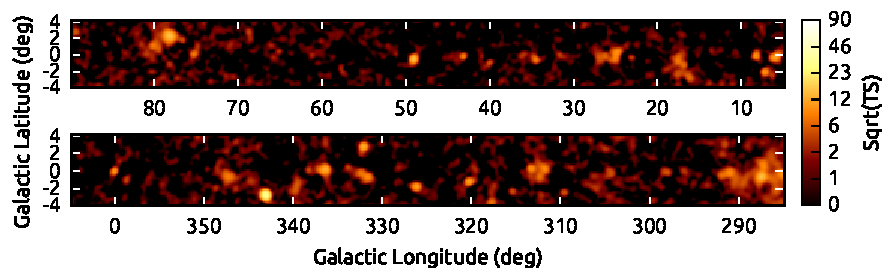
\includegraphics[width=1.\textwidth]{figures/gammapy-fermi-ts-image}
\caption{
Gammapy application example: A \textit{Fermi} survey TS map of the inner
Galactic plane region.
}
\label{fig:fermi-ts-image}
\end{figure*}

\subsection{Morphology analysis}
\label{apps:morph}

\subsection{Spectral analysis}
\label{apps:spec}

\subsection{Cube analysis}
\label{apps:cube}

Maybe. Optional section.

\begin{figure*}[t]
\centering
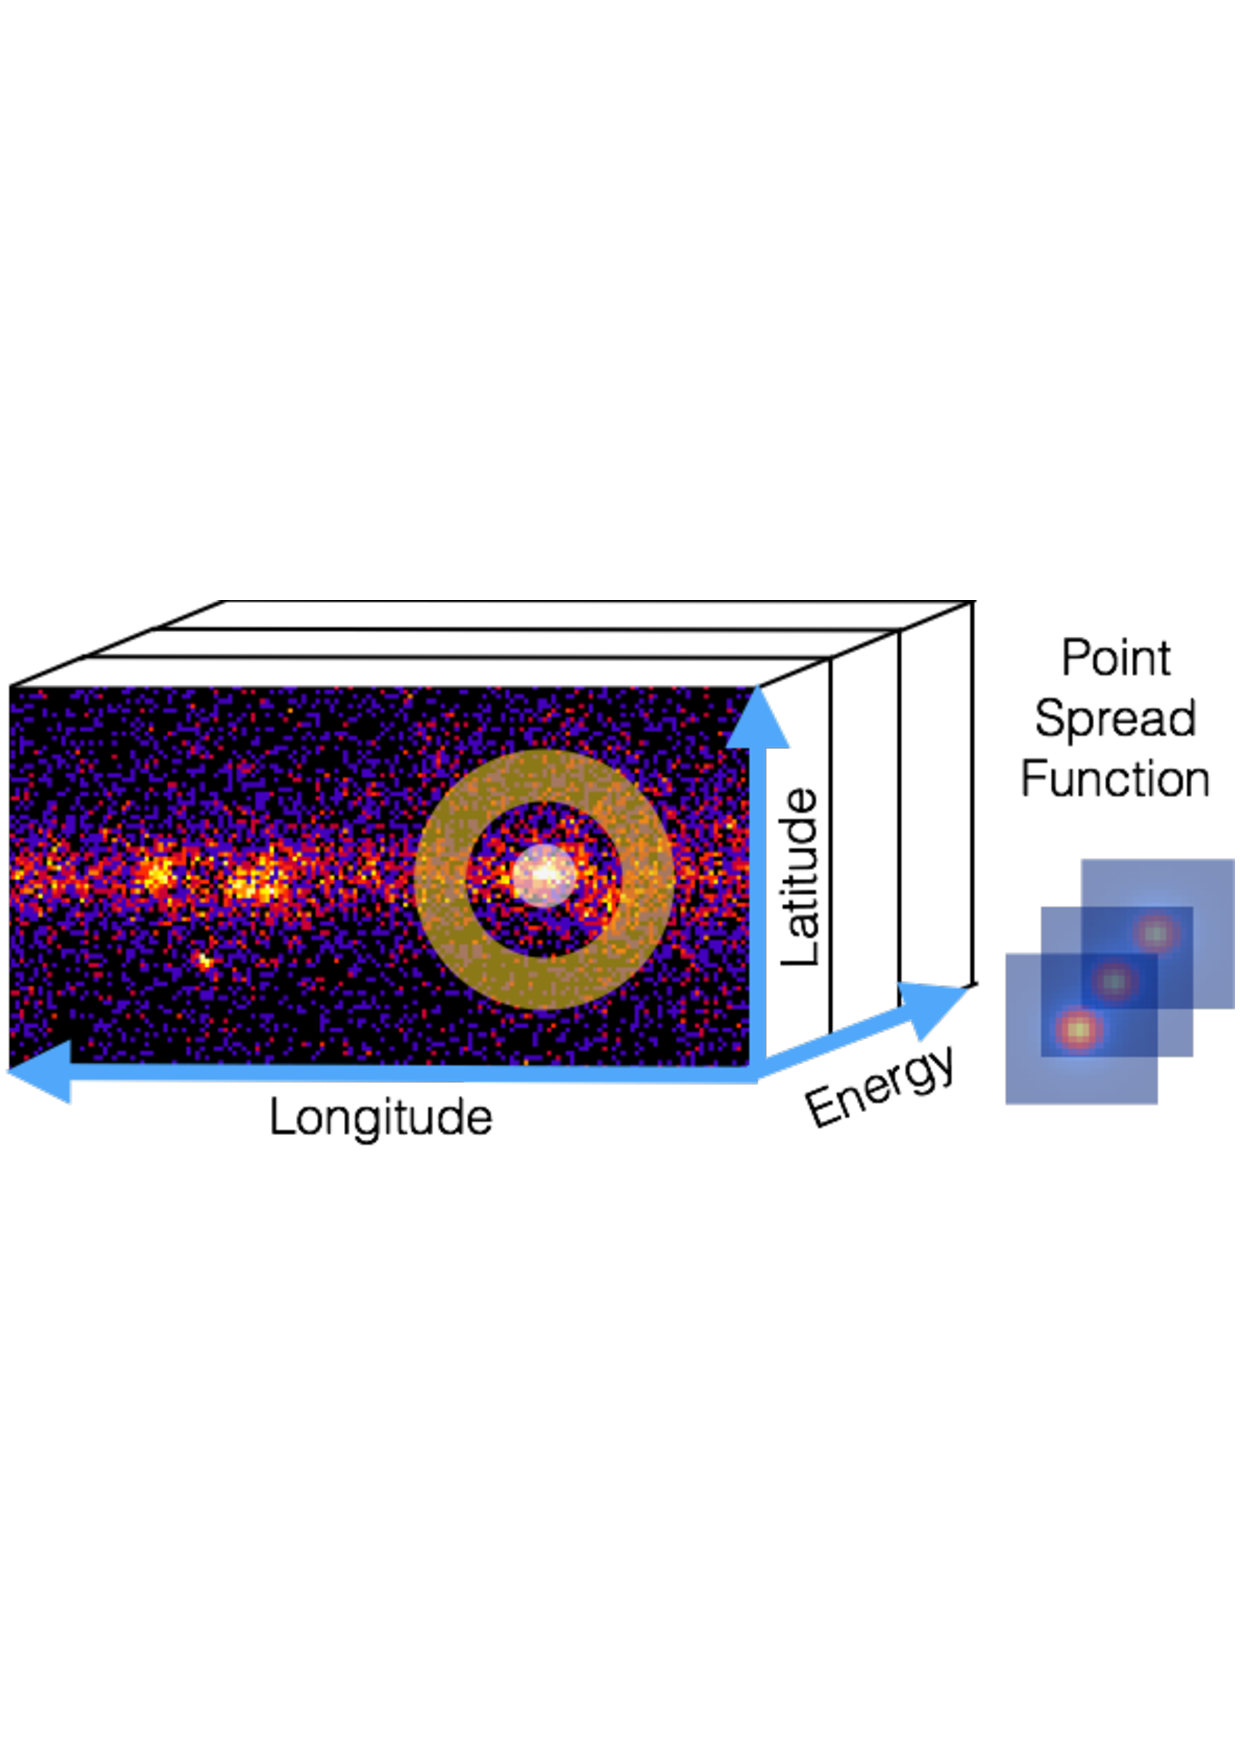
\includegraphics[width=0.8\textwidth]{figures/gammapy-cube-analysis}
\caption{
Gammapy data model illustration. Binned analysis of lon-lat-energy cube data is
supported via joint likelihood analysis of one image per energy bin.
On-off-region based spectral analysis is supported as well.
}
\label{fig:data-model}
\end{figure*}

\subsection{CTA simulation}
\label{apps:sim}

Maybe. Optional section
